\chapter{Semantic Web Practice} \label{ch:semanticwebpractice}

The knowledge in a semantic web is stored using RDF/RDFS and OWL on Turtle, JSON-LD, RDF/XML, or any other media as the developer prefers. To execute an operation such as a query on the semantic web, a database engine is required. The database engines that manage RDF/RDFS and OWL based semantic webs are called triplestore, which is introduced in this chapter.

\section{Triplestore}

Triplestore is the DBMS of RDF/RDFS and OWL. 

When it comes to relational database, there are many choices of DBMS such as Microsoft DBMS, Oracle DBMS, MySQL, MariaDB, and many more. Similarly, there are many choices of triplestore for semantic web. To name a few, a list of widely used triplestores is given below.
\begin{itemize}
	\item GraphDB: a commercialized enterprise-tier semantic graph database management system compliant with W3C standards. It is famous for its performance and inference capabilities. It also provides free-tier for learning and for small projects, with limited capability.
	\item Apache Jena: an open-source Java framework for building semantic web and linked data applications. It has RDF APIs that can read and process RDF and SPARQL written in XML, Turble, JSON-LD and N-Triples.
	\item Virtuoso: a multi-model DBMS for both RDB and NoSQL databases such as RDF. It is famous for its scalability and standards compliance.
	\item Many more, such as Stardog, Blazegraph, AllegroGraph, etc.
\end{itemize}

For the demonstrations given in this notebook, GraphDB is used, unless otherwise mentioned. A full instruction on using GraphDB, including applying for access and installation of the software, can be found at \textit{graphdb.ontotext.com}.

Notice that RDF/RDFS/OWL/SPARQL APIs can be enabled using packages or libraries of many programming languages. For example, in Python, there are several packages available for semantic web operations, including \verb|rdflib|, \verb|Owlready2|, \verb|SPARQLWrapper|, etc. Some of these packages have ``lite'' triplestore engine built-in which provides some SPARQL features for in-memory operations. They do not have all the features of a triplestore. However, they can connect to a triplestore API, in which case they serve as Python-to-triplestore interfaces.  

\section{Example: Semantic Web for Home Assets}

As an example, we are creating a semantic web for a the assets in a household. Here ``assets'' refer to the electrical products, furniture, LEGOs, and other non-consumable, relatively static elements. 

We will start with defining classes to divide everything into large groups, including electrical product, furniture, toy, etc. Under each class, sub-classes are defined, such as TV, computer, game console under electrical product, bed, chair, sofa, lamp under furniture, and LEGO under toy. Lastly, we will define instances under each sub-class. For example, bedroom TV and living room TV under TV, Nintendo SWITCH under game console, living room sofa under sofa, study computer, living room computer, TV attached computer under computer, etc.

We will then use RDFS to enforce schema to the RDF model as follows. Consider electrical product class for example. All elements in this class shall have a property called "hasBrand", which maps them to a pre-defined "electricalBrand" class, inside which are commonly seen electrical brands such as Boche, Siemens, Nintendo, Sony, Google, etc. The electrical product shall also have a "hasPrice" property, "warrantyExpiresAt" property, etc. The similar concept applies to all other produces including furniture, etc.

Finally, use OWL to setup some limits of the properties. For example, for electrical products, the price is usually between 0 to 5000 dollars, etc.

The result should be something like Fig. \ref{fig:houseassetexp}, after visualization.

\begin{figure}[htbp]
	\centering
	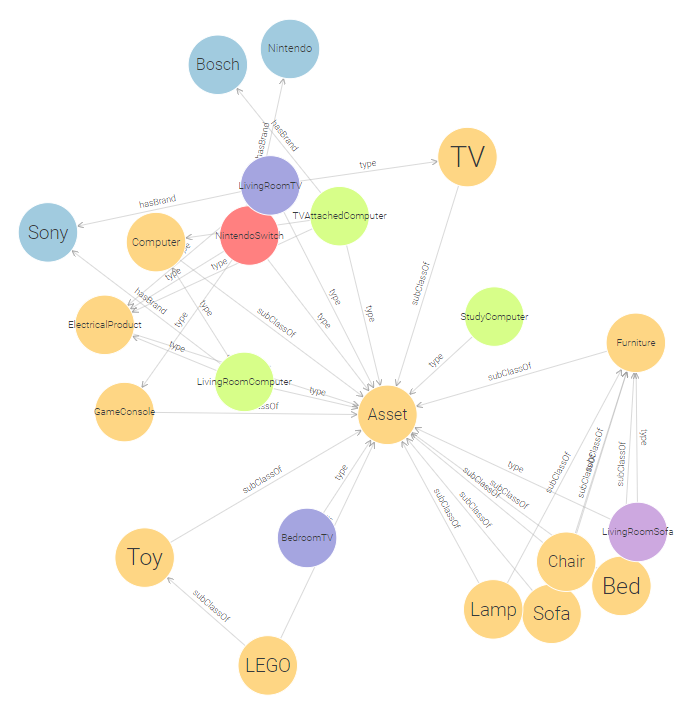
\includegraphics[width=\textwidth]{./chapters/ch-semanticwebpractice/figures/house_asset_exp.png}
	\caption{An example of an RDF model in GraphDB that describes house assets. This is only a demonstration graph and the information inside is artificial and not true.}
	\label{fig:houseassetexp}
\end{figure}

\subsection{Define Classes Hierarchy}

\subsection{Define Properties Hierarchy}

\subsection{Add OWL}

\subsection{Data Retrieval Examples}






